\begin{frame}[parent={cmap:software-testing-foundations}, hasprev=false, hasnext=true]
\frametitle{Erro de taxonomia}
\framesubtitle{Falhas}
\label{concept:falhas}

\begin{block:concept}{O que é uma falha?}
Uma falha é uma definição de dados, passos ou processos incorretos em um software. 
\end{block:concept}

\begin{block:fact}{Como uma falha é criado?}
\begin{itemize}
	\item Uma falha é inserido por um erro.
\end{itemize}
\end{block:fact}

\hfill
\refie{example:incorrect-statement-2}{\beamerbutton{Example: Declaração incorreta}}
\end{frame}



\begin{frame}[hasprev=true, hasnext=true]
\label{concept:mistake}
\frametitle{Erro de taxonomia}
\framesubtitle{Erro}

\begin{block:concept}{O que é um erro?}
Um erro é uma ação humana que produz um resultado incorreto.
\end{block:concept}

\begin{block:fact}{Como um erro ocorre?}
\begin{itemize}
	\item Pela falta de atenção durante a execução de um software?

	\item Pela omissão de informações na especificação de requisitos do software?

	\item Erro de compilação (ocasionado por um erro)?
\end{itemize}
\end{block:fact}

\hfill
\refie{example:incorrect-statement-1}{\beamerbutton{Example: Declaração incorreta}}
\end{frame}



\begin{frame}
\label{concept:error}
\frametitle{Erro de taxonomia}
\framesubtitle{Error}

\begin{block:concept}{O que é um erro?}
An error is the difference between a computed, observed or measured value
or condition and the true, theoretically correct or specified value or
condition.
\end{block:concept}

\begin{block:fact}{Como um erro ocorre?}
\begin{itemize}
	\item Um erro é produzido pela execução de uma falha.
	\begin{itemize}
		\item Assim, se uma falha nunca é executada, ele nunca produz um erro.
	\end{itemize}
\end{itemize}
\end{block:fact}
\end{frame}


\begin{frame}
\label{concept:failure}
\frametitle{Erro de taxonomia}
\framesubtitle{Falha}

\begin{block:concept}{O que é uma falha?}
Uma falha é a incapacidade de um componente ou um sistema de cumprir suas funções necessárias dentro dos requisitos de desempenho especificados.
\end{block:concept}

\begin{block:fact}{Como uma falha ocorre?}
\begin{itemize}
	\item Uma falha e seus erros associados podem causar uma ou mais falhas.
\end{itemize}
\end{block:fact}

\hfill
\refie{example:incorrect-statement-3}{\beamerbutton{Example: Declaração incorreta}}
\end{frame}



\begin{frame}
\frametitle{Erro de taxonomia}

\begin{block:procedure}{Summary}
\begin{enumerate}
	\item Um programador comete um \textbf{erro}.
	\begin{itemize}
		\item Um único $<$ passa a ter um $>$ em uma única instrução.
	\end{itemize}

	\item Devido ao erro, a declaração está com \textbf{falha} (não implementar o comportamento descrito na especificação de requisitos de software).

	\item O software é compilado e executado. A instrução fornecida é executada. Como ele pertence a uma função responsável pela criação da soma de verificação dos dados que estão sendo processados, a saída que é produzida é incorreta (\textbf{erro}).

	\item O usuário compara a soma de verificação produzido pelo software com o resultado esperado. Não importa o que, a soma de verificação sempre \textbf{falha}.
\end{enumerate}
\end{block:procedure}
\end{frame}



\begin{frame}[c, hasprev=true, hasnext=false]
\label{concept:defect-taxonomy}
\frametitle{Erro de taxonomia}

\begin{block:fact}{}
    \centering
    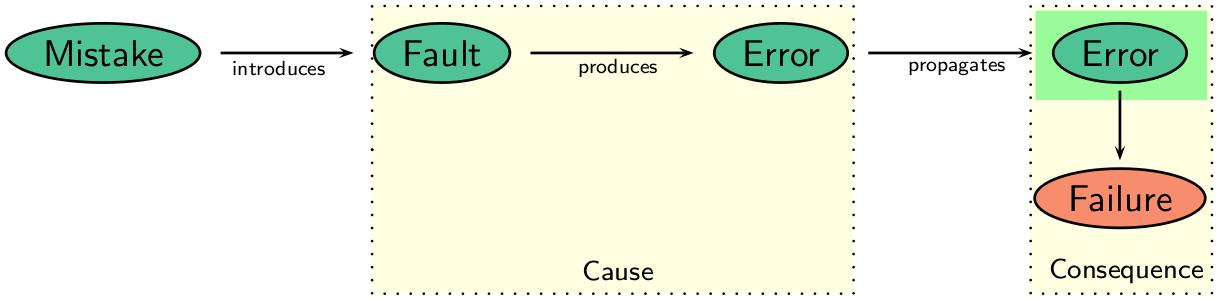
\includegraphics[scale=.3]{teste-de-software/conceitos-basicos/Imagens/defect-taxonomy}
\end{block:fact}

\hfill
\refie{example:physician-analogy-for-defect-taxonomy}{\beamerbutton{Example: Physician analogy for defect taxonomy}}
\refie{example:numzero}{\beamerbutton{Example: Exemplo de erro de taxonomia (numZero)}}
\end{frame}
